\newpage
\section{Hotspot Analysis}

The Fourier Transform is a fundamental mathematical tool in digital signal processing. 
It converts a sequence of values from the \textbf{time domain} into a sequence of values in the \textbf{frequency domain}. 
This transformation makes it possible to identify which frequencies are present in a signal and with what intensity.\\

\noindent
The continuous-time Fourier Transform is defined as:
\[
X(\omega) = \int_{-\infty}^{+\infty} x(t)\, e^{-j \omega t}\, dt
\]

\noindent
The example shown in Figure \ref{fig:rectangle_fourier_transform} illustrates the practical and optical interpretation of the Fourier Transform of a rectangular signal, showing how a simple time–domain shape corresponds to a characteristic frequency–domain spectrum.

\begin{figure}[ht]
    \centering
    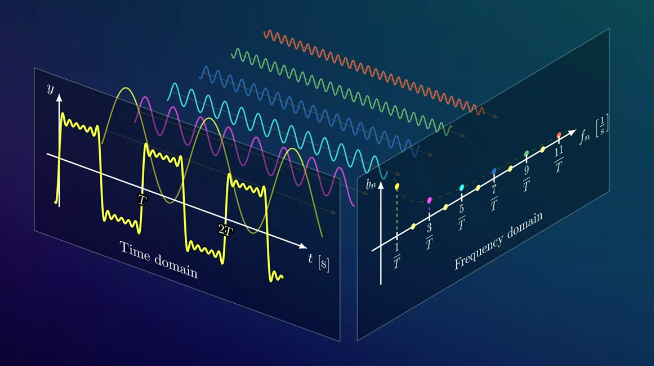
\includegraphics[width=0.9\textwidth]{assets/hotspots/rectangle_fourier_transform.png}
    \caption{Fourier Transform of a rectangular signal.}
    \label{fig:rectangle_fourier_transform}
\end{figure}

\subsection{Code Description}
The algorithm provided by the course implements both the Discrete Fourier Transform (DFT) and its inverse (IDFT) in C. 
It computes the transform of a signal and verifies the correctness by applying the IDFT, following the discrete-time Fourier Transform definition:

\[
X[k] = \sum_{n=0}^{N-1} x[n] \, e^{-j 2 \pi k n / N}, 
\quad k = 0,1,\dots,N-1
\]

\noindent
The DFT is implemented following the standard quadratic-complexity $O(N^2)$ formulation, with two nested loops 
over the frequency index $k$ and the time index $n$. Each output element can be 
computed independently, which makes the algorithm naturally parallelisable.

\begin{lstlisting}[caption={Pseudo code in C}]
int main() {
    int N = 100000;
    double *xr, *xi, *Xr, *Xi;

    fillInput(xr, xi, N);            // initialize input signal
    zero(Xr, Xi, N);                 // clear output buffers

    DFT(+1, xr, xi, Xr, Xi, N);      // compute DFT
    DFT(-1, Xr, Xi, xr, xi, N);      // compute IDFT

    checkResults(xr, xi, Xr, Xi, N); // verify correctness

    return 0;
}

void DFT(int idft, double* xr, ..., double* Xi, int N) {
    for (int k = 0; k < N; k++)
        for (int n = 0; n < N; n++) {
            double a = 2*M_PI*n*k/N;
            Xr[k] += xr[n]*cos(a) + idft*xi[n]*sin(a);
            Xi[k] += -idft*xr[n]*sin(a) + xi[n]*cos(a);
        }

    if (idft == -1)
        for (int n = 0; n < N; n++) {
            Xr[n] /= N;
            Xi[n] /= N;
        }
}
\end{lstlisting}

\subsection{Project Structure}
The \texttt{homework1} project is organized into four main directories:
\begin{itemize}
    \item \textbf{build}: contains the compiled executables.
    \item \textbf{reports}: stores the reports generated with the \texttt{-qopt-report} flag.
    \item \textbf{src}: includes the source code files.
    \item \textbf{metrics}: scripts that run the executables in \texttt{build} and save performance metrics.
\end{itemize}

\noindent
The first step to improving the performance of a program is profiling. The goal of this analysis is to identify the parts of the program that consume the most execution time. To achieve this, I considered a data size resulting in a sequential execution time of $\sim 30$ seconds, by setting $N = 60'000$.\\

\noindent
From this point onward, each executable is empirically measured over 10 runs to obtain reliable results.


\subsection{Sequential and Parallel Sections}
In order to apply Amdahl's Law (discussed in more detail in the Chapter~\ref{sec:amdahls_law}), we must identify the sequential and parallel parts of the code. 
I have empirically measured these sections by separating the serial and parallel portions.
More details of how I obtained these results can be found in the code \texttt{sequential\_parallel\_code\_identification.c}.\\

\noindent
The results are the following:

% TODO aggiungere i valori
\begin{table}[h!]
\centering
\begin{tabular}{l c}
\hline
\textbf{Quantity} & \textbf{Value} \\
\hline
Total execution time $T_\text{tot}$ & $\text{32.48231}$ s \\
Time of the parallelizable section $T_\text{par}$ & $\text{32.48021}$ s \\
Time of the serial section $T_\text{ser} = T_\text{tot} - T_\text{par}$ & $\text{0.00209}$ s \\
Fraction of serial code $f_s = \frac{T_\text{ser}}{T_\text{tot}}$ & $\text{0.006}$ \% \\
\hline
\end{tabular}
\label{tab:seq_par_times}
\end{table}

\noindent
These values will be used to estimate the theoretical speedup according to Amdahl's Law:

\[
S(p) = \frac{1}{f_s + \frac{1-f_s}{p}} \Big|_{f_s=0.00006} =  \frac{1}{0.00006 + \frac{1-0.00006}{p}} \approx p
\]

\paragraph{Note:} the smaller the serial fraction $f_s$, the higher the potential speedup achievable by parallelizing the main loop of the DFT.

\paragraph{Note: in the real case, the speedup is not linear.}
In particular, from the parallelization examples presented in Chapter~\ref{sec:parallelization}, the speedup is approximately linear up to 8 threads; beyond this point, it deviates from linear behavior.

\subsection{Compilation}
Since the Intel(R) C++ Compiler Classic (ICC) is deprecated and was removed from product release in the second half of 2023. The Intel(R) oneAPI DPC++/C++ Compiler (ICX) was used to performe the analysis.\\
\\
To identify the optimal sequential compilation strategy, I conduced testing across multiple Intel compiler variants (\texttt{ICC} and \texttt{ICX}), focusing on the vectorization report provided by the flag \texttt{-qopt-report}.\\
The program was compiled using the Intel compiler \texttt{ICX} with the following command (more details in Chapter~\ref{sec:vectorization}):
\begin{verbatim}
icx -O2 -vec -g \
    -fopenmp \
    -qopt-report=max \
    -qopt-report-file=reports/omp_homework.optrpt \
    -o build/omp_homework \
    src/omp_homework.c
\end{verbatim}

The compilation flags have the following meaning:
\begin{itemize}
    \item \texttt{-O2}: optimizations for better performance;
    \item \texttt{-fopenmp}: activates compilation for OpenMP directives;
    \item \texttt{-vec}: activates automatic vectorization of loops using SIMD instructions;
    \item \texttt{-g}: includes debugging information in the executable;
    \item \texttt{-qopt-report=max}: generates a detailed optimization report;
    \item \texttt{-qopt-report-file=...}: specifies the file where the optimization report is saved;
    \item \texttt{-o build/omp\_homework}: sets the name and location of the compiled executable;
    \item \texttt{src/omp\_homework.c}: specifies the source file to compile.
\end{itemize}


\subsection{Hotspot Identification}
The measurements were performed using two methods: \textbf{Manually} (using \texttt{omp\_get\_wtime()}) and \textbf{Profiler} (using \texttt{Intel VTune})

% TODO: aggiornare le tabelle
\begin{table}[htbp]
\centering
\begin{minipage}{0.48\textwidth}
    \centering
    \caption{Manually}
    \resizebox{\textwidth}{!}{%
    \begin{tabular}{lrr}
        \toprule
        Function & Time (s) & Percentage (\%) \\
        \midrule
        \csvreader[late after line=\\]{assets/hotspots/hotspots_identification.csv}{}
        {\csvcoli & \csvcolii & \csvcoliii} 
        \bottomrule
    \end{tabular}%
    }
\end{minipage}%
\hfill
\begin{minipage}{0.48\textwidth}
    \centering
    \caption{Intel VTune Profiler}
    \resizebox{\textwidth}{!}{%
    \begin{tabular}{lrr}
        \toprule
        Function Stack & CPU Time: Total & Percentage (\%) \\
        \midrule
        \csvreader[late after line=\\]{assets/hotspots/top-down-tree.csv}{}
        {\csvcoli & \csvcolii & \csvcoliii} 
        \bottomrule
    \end{tabular}%
    }
\end{minipage}
\end{table}

\begin{center}
    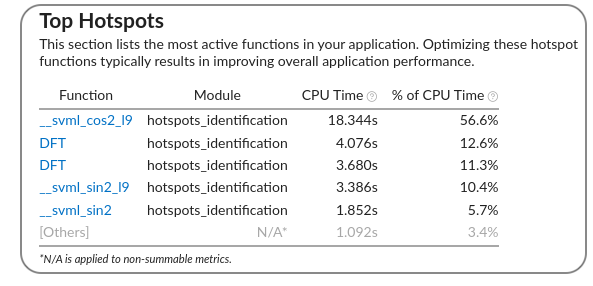
\includegraphics[width=0.8\textwidth]{assets/hotspots/top_hotspots_vtune.png}
\end{center}

\subsection{Conclusions}
The main hotspot is the DFT() function and its inverse IDFT(), which together account for over 99,05\% of the total execution time. All other functions have negligible impact. This indicates that \textbf{parallelization and vectorization efforts should focus on the double loop inside DFT()}.\\

\noindent
\textbf{The main hotspot is the loop contained in lines 72-80 (source: \texttt{src/omp\_homework.c})}. The dominant operations contributing to the algorithm's computational intensity are the \texttt{sin()} and \texttt{cos()} trigonometric functions, which account for the majority of the execution time, as shown in the following code.

\begin{figure}[ht]
    \centering
    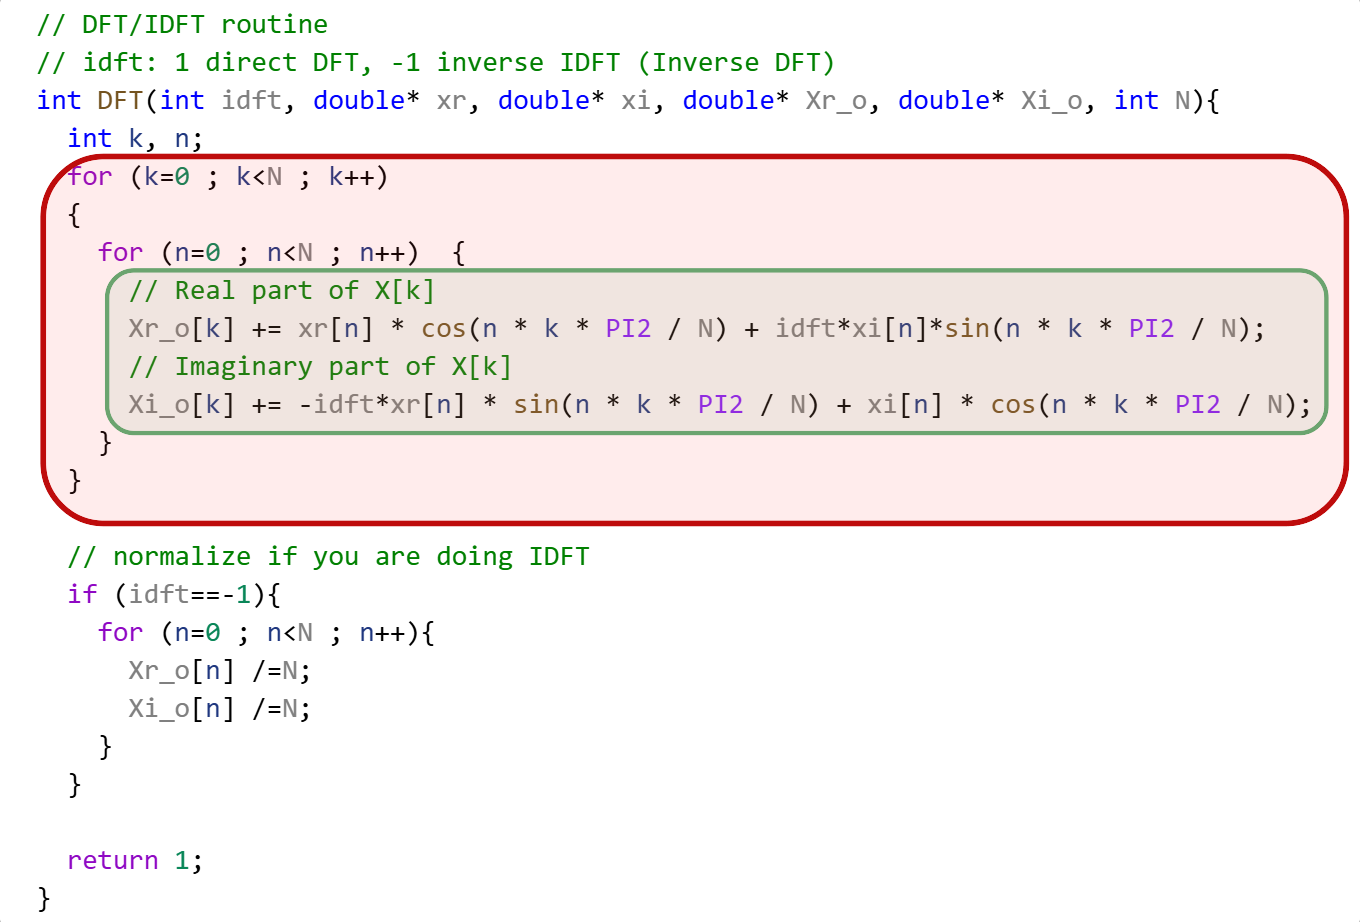
\includegraphics[width=0.9\textwidth]{assets/hotspots/hotspot_code_evidentiation.png}
    \label{fig:vtune_biggest_hotspot_screen}
\end{figure}
